\chapter{Описание реализации метода частиц в ячейках для высокопроизводительных ВС}
\label{chapt1}

\section{Краткое описание метода частиц в ячейках}
\label{beam-plasma-methods}


Основываясь на
\cite{VshivkovPICbook}, приведем описание основной идеи метода. Пусть задача записана 
в абстрактной операторной форме:
\begin{equation}
\label{Abs1}
\frac{\partial \textbf{q}}{\partial t} + A\textbf{q} = 0.
\end{equation}

Решение задачи (\ref{Abs1}) представляется в виде следующей интерполяционной 
формулы:
\begin{equation}
\label{AbsInt}
\textbf{q} = \sum\limits^{N}_{j=1}\textbf{Q}_j R(\textbf{u},\textbf{u}_j(t)).
\end{equation}
Этот переход называют разбиением среды на модельные частицы. Функция 
$R(\textbf{u},\textbf{v})$ называется ядром модельной частицы. Представление
(\ref{AbsInt}) позволяет свести решение задачи 
(\ref{Abs1}) к интегрированию динамической системы частиц.


\quad Система уравнений движения модельных частиц получается, как указано в книге
\cite{VshivkovPICbook} из уравнения Власова подстановкой функции
распределения в виде
\begin{equation}\label{fr}
f(t,x,u)=\sum_{j=1}^m R(x-x_j(t))\delta(u-u_j(t))
\end{equation}
где $R$ -- произвольное сеточное ядро,  %ядро модельной частицы,
$\delta$ -- дельта-функция, $m$ -- полное число модельных частиц.

Для удобства будем рассматривать наши уравнения в безразмерных
величинах
\begin{equation}\label{dx}
\frac{dx_j(t)}{dt}=u_j(t),
\end{equation}
\begin{equation}\label{du}
\frac{du_j(t)}{dt}=E(x_j),
\end{equation}
\begin{displaymath}
j=1,\ldots, m
\end{displaymath}
- уравнения движения частиц (совпадают с уравнениями характеристик
кинетического уравнения Власова).

\section{Модель высокотемпературной бесстолкновительной плазмы}

Математическая модель высокотемпературной бесстолкновительной плазмы
представляется кинетическим уравнением Власова и системой
уравнений Максвелла \cite{VshivkovPICbook,birdsall2004plasma}, которые в безразмерной форме имеют
следующий вид:

\begin{equation}\label{eq:Vlas}
\frac{\partial f_{i,e}}{\partial t}+{\textbf{v}} \frac{\partial f_{i,e}}{\partial \textbf{r}}+q_{i,e}({\textbf{E}}+[{\textbf{v}},{\textbf{B}}])\frac{\partial f_{i,e}}{\partial \textbf{v}}=0, 
\end{equation}

\begin{eqnarray}
& \frac{\partial \textbf{E}}{\partial t}=rot \textbf{B} - \textbf{j}, & \label{eq:dE}
\\
& \frac{\partial \textbf{B}}{\partial t}=-rot \textbf{E}, & \label{eq:dB}
\\
& div \textbf{E} = \rho, & \label{eq:divE}
\\
& div \textbf{B} = 0. & \label{eq:divB}
\end{eqnarray}

Здесь индексами $i$ и $e$ помечены величины, относящиеся к ионам и
электронам, со\-от\-ветст\-вен\-но; $q_e=-1, \quad q_i=m_e/m_i$; $f_{i,e}(t,\textbf{r},\textbf{p})$ --
функция распределения частиц; $m_{i,e}, \textbf{p}_{i,e},
\textbf{r}_{i,e}$ -- масса, импульс, положение иона или электрона;
$\textbf{E}$, $\textbf{B}$ -- напряженности электрического и магнитного
полей. Для перехода к безразмерному виду в качестве единиц
используются следующие базовые величины:(скорость света $c$, масса электрона,
\begin{itemize}
\item плотность плазмы $n_0=10^{14}$ см $^{-3}$,
\item время $t=\omega _{pe}^{-1}$, где плазменная электронная частота $\omega_{pe} =5,6 \cdot 10^{11}$c$^{-1}$)
\end{itemize}

%\bibliographystyle{gost2008}
%\bibliography{biblio/snytav_othercites,biblio/lotov_plasma,biblio/exaflops_related1,biblio/snytav_papersVAK,biblio/snytav_review,biblio/exaflops_related}
%\end{document} 	

%Все уравнения приводятся в безразмерном виде.

В начальный момент времени в трехмерной области
решения, имеющей форму прямоугольного параллелепипеда $$
x\in[0,L],\quad y,z\in[0,L_\bot], $$ находится плазма, состоящая из
электронов и ионов водорода, и пучок электронов. Заданы плотности электронов пучка $n_b$ и электронов плазмы $n_e = 1-n_b$. Плотность ионов плазмы в рамках используемой в данной работе модели, подробнее описанной в \cite{VychMetPlasma} равна сумме плотностей электронов пучка и электронов плазмы. Температура электронов плазмы $T_e$ и пучка $T_b$; температура ионов считается нулевой $T_i=0$. Начальное распределение частиц по скоростям макс\-вел\-ловс\-кое с плотностью распределения

$$
f(v)=\frac{1}{\Delta v \sqrt{2
		\pi}}\exp \left( {-\frac{(v-v_0)^2}{2 \Delta v^2}}\right) ,
$$
где $\Delta v$ -- разброс частиц по скоростям ($T_b=\Delta v^2$), $v_0$ -- средняя
скорость пучка. Средняя скорость ионов и электронов фона нулевая. Все частицы распределены по области равномерно, начальная средняя скорость пучка направлена по $x$ и равна $v_0=0.2$. Граничные условия периодические. 





%В зависимости от разброса электронов пучка по скоростям различают несколько режимов неустойчивости, как показано в таблице \ref{tab_regimes}. Здесь $\gamma$ --  инкремент развивающейся неустойчивости, $\Delta v $ -- разброс электронов пучка по скоростям. Требуется найти распределение ионов и электронов по энергиям и инкременты плазменной неустойчивости для физических параметров, соответствующих этим трем режимам.



\section{Решение уравнений Максвелла и Власова}

Решение уравнения Власова проводится методом
частиц-в-ячейках \cite{hockney, birdsall2004plasma,VshivkovPICbook}. Плазма представляется набором модельных частиц, траекториями движения которых являются характеристики урав\-не\-ния Власова

\begin{equation}\label{eq:char}
\begin{array}{c}
\frac{d {\textbf{p}} _{e}}{d t}=-(\textbf{E}+[\textbf{v},\textbf{B}]), \\
\frac{d {\textbf{p}} _{i}}{d t}=k(\textbf{E}+[\textbf{v},\textbf{B}]), \\
\frac{d {\textbf{r}} _{i}}{d t}={\textbf{v}}_{i}.
\end{array}
\end{equation}


Для решения системы уравнений (\ref{eq:char}) используется схема
$$
\frac{{\textbf{p}}^{m+1/2}_{i}-{\textbf{p}}^{m-1/2}_{i}}{\tau}=q_{i}\left({\textbf{E}}^m+\left[\frac{{\textbf{v}}^{m+1/2}_{i}+{\textbf{v}}^{m-1/2}_{i}}{2},{\textbf{B}}^m \right] \right),
$$
$$
\frac{{\textbf{r}}_{i}^{m+1}-{\textbf{r}}_{i}^{m}}{\tau}={\textbf{v}}^{m+1/2}_{i}.
$$


Плотность заряда вычисляется по положениям частиц ${\textbf{r}}_\alpha=(x_\alpha,y_\alpha,z_\alpha)$ с использованием PIC-ядра 
$$
\rho({\textbf{r}}, t)=\sum_{j=1}^J q_{j} R({\textbf{r}}, {\textbf{r}}_{j}(t)),
$$

\begin{equation}
R(x)=\left\{
\begin{array}{ll}
\displaystyle \frac{1}{h}\left(1-\frac{|x|}{h}\right), & |x|\leq h, \\ 0, & |x|>h.
\end{array} \right.
\end{equation}

Для решения системы уравнений Максвелла используется метод Лэнгдона-Лазински, описанный в работе \cite{lasin}, в котором поля определяются из разностных аналогов законов Фарадея и Ампера:

\begin{equation}
\begin{array}{c}
\frac{{\textbf{B}}^{m+1/2}-{\textbf{B}}^{m-1/2}}{\tau}=-\rot_h {\textbf{E}}^m,
\\
\frac{{\textbf{E}}^{m+1}-{\textbf{E}}^m}{\tau}=\rot_h {\textbf{B}}^{m+1/2} - {\textbf{j}}^{m+1/2}.
\end{array}
\label{FDTD}
\end{equation}
Значения компонент напряженностей электрического и магнитного полей вычисляются в узлах сеток, смещенных относительно друг друга по времени и пространству:
\begin{equation}
\label{eq:BE}
\begin{array}{c}


{\textbf{B}}^{m+1/2}=(B^1_{i+1/2,j,l}, B^2_{i,j+1/2,l}, B^3_{i,j,l+1/2})^{m+1/2},
\\
{\textbf{E}}^{m}=(E^1_{i,j+1/2,l+1/2}, E^2_{i+1/2,j,l+1/2}, E^3_{i+1/2,j+1/2,l})^m,
\\
{\textbf{j}}^{m+1/2}=(j^1_{i,j+1/2,l+1/2},j^2_{i+1/2,j,l+1/2},j^3_{i+1/2,j+1/2,l})^{m+1},
\\
\rho^m=\rho^m_{i+1/2,j+1/2,l+1/2}. 
\end{array}
\end{equation}

Разностные операторы $\rot_h$ и $\diver_h$ на такой сетке имеют следующий вид (в индексах опустим $1/2$)
\begin{equation}
\label{eq:rotdiv}
\rot_h { \textbf{H}} =  \left(\begin{array}{c}  \frac{H^3_{i,j,l}-H^3_{i,j-1,l}}{h_y}-\frac{H^2_{i,j,l}-H^2_{i,j,l-1}}{h_z}, 
\\
\frac{H^1_{i,j,l}-H^1_{i,j,l-1}}{h_z}-\frac{H^3_{i,j,l}-H^3_{i-1,j,l}}{h_x},  
\\
\frac{H^2_{i,j,l}-H^2_{i-1,j,l}}{h_x}-\frac{H^1_{i,j,l}-H^1_{i,j-1,l}}{h_y} \end{array} \right) 
\\
\end{equation}
\begin{equation}
\diver_h { \textbf{H}} =  \frac{H^1_{i+1,j,l}-H^1_{i,j-1,l}}{h_x}+\frac{H^2_{i,j+1,l}-H^2_{i,j,l}}{h_y}+\frac{H^3_{i,j,l+1}-H^3_{i,j,l}}{h_z}. 
\end{equation}

Эта схема имеет порядок аппроксимации $O(\tau^2+h^2)$. Если в начальный момент времени $\diver_h{\textbf{B}}^0=0$, а токи вычисляются таким образом, что выполнено уравнение неразрывности 

\begin{equation}
\frac{\rho^{m+1}-\rho^m}{\tau}+\diver_h {\textbf{j}}^{m+1/2}=0,
\end{equation}
то разностные аналоги уравнений (\ref{eq:divE}) и (\ref{eq:divB}) выполняются автоматически.
Для того, чтобы удовлетворить этим условиям, токи вычисляются по схеме, приведенной в работах \cite{VshivkovPICbook, laser}, ${\textbf{B}}^0=0$. 

Компоненты плотности тока \textbf{j}
\begin{equation}
\begin{array}{c}
%\begin{center}
j_{x,i,l-1/2,k-1/2}^{m+1/2}=q\frac{\Delta x}{\tau}\left[(1-\delta_{y})(1-\delta_{z})+\dfrac{\Delta y \Delta z}{12 h_{y}h_{z}}
\right], \\
j_{x,i,l-1/2,k+1/2}^{m+1/2}=q\frac{\Delta x}{\tau}\left[(1-\delta_{y})\delta_{z}-\dfrac{\Delta y \Delta z}{12 h_{y}h_{z}}
\right], \\
j_{x,i,l+1/2,k-1/2}^{m+1/2}=q\frac{\Delta x}{\tau}\left[\delta_{y}(1-\delta_{z})-\dfrac{\Delta y \Delta z}{12 h_{y}h_{z}}
\right], \\
j_{x,i,l+1/2,k+1/2}^{m+1/2}=q\frac{\Delta x}{\tau}\left[\delta_{y}\delta_{z}+\dfrac{\Delta y \Delta z}{12 h_{y}h_{z}}
\right], \\
j_{y,i-1/2,l,k-1/2}^{m+1/2}=q\frac{\Delta y}{\tau}\left[(1-\delta_{x})(1-\delta_{z})+\dfrac{\Delta x \Delta z}{12 h_{x}h_{z}}
\right], \\
j_{y,i-1/2,l,k+1/2}^{m+1/2}=q\frac{\Delta y}{\tau}\left[(1-\delta_{x})\delta_{z}-\dfrac{\Delta x \Delta z}{12 h_{x}h_{z}}
\right], \\
j_{y,i+1/2,l,k-1/2}^{m+1/2}=q\frac{\Delta y}{\tau}\left[\delta_{x}(1-\delta_{z})-\dfrac{\Delta x \Delta z}{12 h_{x}h_{z}}
\right], \\
j_{y,i+1/2,l,k+1/2}^{m+1/2}=q\frac{\Delta y}{\tau}\left[\delta_{x}\delta_{z}+\dfrac{\Delta x \Delta z}{12 h_{x}h_{z}}
\right] \\
j_{z,i-1/2,l-1/2,k}^{m+1/2}=q\frac{\Delta z}{\tau}\left[(1-\delta_{x})(1-\delta_{y})+\dfrac{\Delta x \Delta y}{12 h_{x}h_{y}}
\right], \\
j_{z,i-1/2,l+1/2,k}^{m+1/2}=q\frac{\Delta z}{\tau}\left[(1-\delta_{x})\delta_{y}-\dfrac{\Delta x \Delta y}{12 h_{x}h_{y}}
\right], \\
j_{z,i+1/2,l-1/2,k}^{m+1/2}=q\frac{\Delta z}{\tau}\left[\delta_{x}(1-\delta_{y})-\dfrac{\Delta x \Delta y}{12 h_{x}h_{y}}
\right], \\
j_{z,i+1/2,l+1/2,k}^{m+1/2}=q\frac{\Delta z}{\tau}\left[\delta_{x}\delta_{y}+\dfrac{\Delta x \Delta y}{12 h_{x}h_{y}}
\right], \\
\end{array}
\end{equation}
где $\Delta x=x_2-x_1;$ $\Delta y=y_2-y_1;$ $\Delta z=z_2-z_1;$ -- приращение координат, индексом 1 обозначена координата частицы до сдвига, индексом 2 - после; 

Более подробно эти вычисления описаны в \cite{VychMetPlasma,MatMod,LotovPoP}


\section{ Параллельная реализация} 


\subsection{Декомпозиция расчетной области}

\begin{figure}[ht]
	\begin{center}
		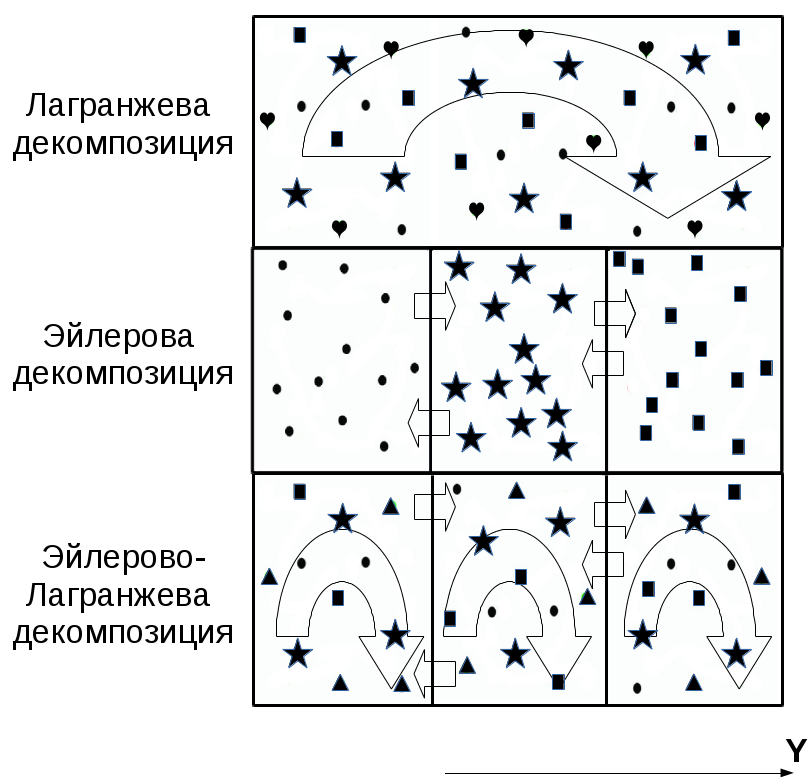
\includegraphics[height=14cm,keepaspectratio]{images/decomp_all_BW_1.png}
	\end{center}
	\caption{Различные варианты декомпозиции расчетной области. На рисунке показано разделение расчетной области на подобласти вдоль одной из координат. Различные символы (круг, квадрат, звезда, треугольник) означают модельные частицы, находящиеся на разных процессорных  элементах. Стрелки означают межпроцессорные коммуникации: прямые стрелки - MPI\_Send и MPI\_Recv, изогнутые  - MPI\_Allreduce.}
	\label{decomp_all_bw}
\end{figure}

Были рассмотрены и реализованы следующие три варианта декомпозиции:

\begin{itemize}
\item \textbf{Лагранжева} декомпозиция: разделение расчетной области (пространства моделирования) между процессорными элементами (ПЭ) на части по количеству подвижных элементов
(разделяются \textbf{частицы}, независимо от координаты) , схематически лагранжева декомпозиция показана на рис. \ref{decomp_all_bw}.

\item \textbf{Эйлерова} декомпозиция: разделение расчетной области (пространства моделирования) между процессорными элементами (ПЭ) на части по координате (ячейки сетки и \textbf{находящиеся в них частицы}, схематически эйлерова декомпозиция показана на рис. \ref{decomp_all_bw}.

\item Смешанная \textbf{Эйлерово-лагранжева} декомпозиция \cite{VychMethProgExa}. Расчетная область разделяется на подобласти для решения уравнений Максвелла, и на каждую подобласть назначается группа из $M$ ПЭ, далее частицы каждой подобласти разделяются дополнительно между этими $M$ ПЭ. Этот вариант декомпозиции показан на рис. \ref{decomp_all_bw}.

\end{itemize}

Эффективность распараллеливания, достигаемая при использовании  этих трех вариантов декомпозиции расчетной области показана в таблице \ref{effcompare}. 



\begin{table}[ht]
\caption{Эффективность в слабом смысле, достигнутая при различных вариантах декомпозиции.}
\begin{center}

\begin{tabular}{|c|c|c|}
\hline
Декомпозиция & тип коммуникаций        &  эффективность (МСЦ РАН) \\
             &                         &  на 100 ПЭ\\ \hline
эйлерова     & <<точка-точка>>         &   77 \%  \\ \hline
 лагранжева  & коллективные            &   15 \%  \\
             &  по всем ПЭ             &        \\ \hline
 смешанная   & <<точка-точка>> и       &   92 \%  \\ 
             & коллективные            &       \\
             & по небольшим            &        \\ 
             & группам ПЭ              &      \\ \hline 
\end{tabular}
\end{center}
\label{effcompare}
\end{table}





Для параллельной реализации метода частиц в ячейках в данной работе используется эйлерово-лагранжева декомпозиция расчетной области. Такой вариант выбран из соображений наилучшей масштабируемости вычислительного алгоритма.
При этом расчетная область разделяется на подобласти для решения уравнений Максвелла, и на каждую подобласть назначается группа из $M$ ПЭ, далее частицы каждой подобласти разделяются дополнительно между этими $M$ ПЭ. Такой вариант декомпозиции одновременно обеспечивает минимизацию фрагмента вычислительного алгоритма и также соответствует условию линейности алгоритма, необходимому для достижения высокой масштабируемости. Этот подход близок к виртуальным слоям (Malyshkin, Kraeva, 2001).

В пользу именно такого, смешанного варианта декомпозиции можно высказать следующие теоретические соображения:
\begin{itemize}
	\item Для эйлеровой декомпозиции минимальным фрагментом (Понятие минимального фрагмент было введено В.Э.Малышкиным, 2001) является слой сетки вместе с частицами
	\item Для лагранжевой декомпозиции минимальный фрагмент - одна частица
	\item Тем не менее, для лагранжевой декомпозиции (из-за необходимости осуществлять коллективные коммуникации по всем ПЭ) нарушается критерий линейности алгоритма (В.Э.Малышкин, 1991)
	\item Эйлерово-лагранжева декомпозиция позволяет одновременно минимизировать размер фрагмента и обеспечить линейность
	
\end{itemize}




\begin{figure}[ht]
\begin{center}
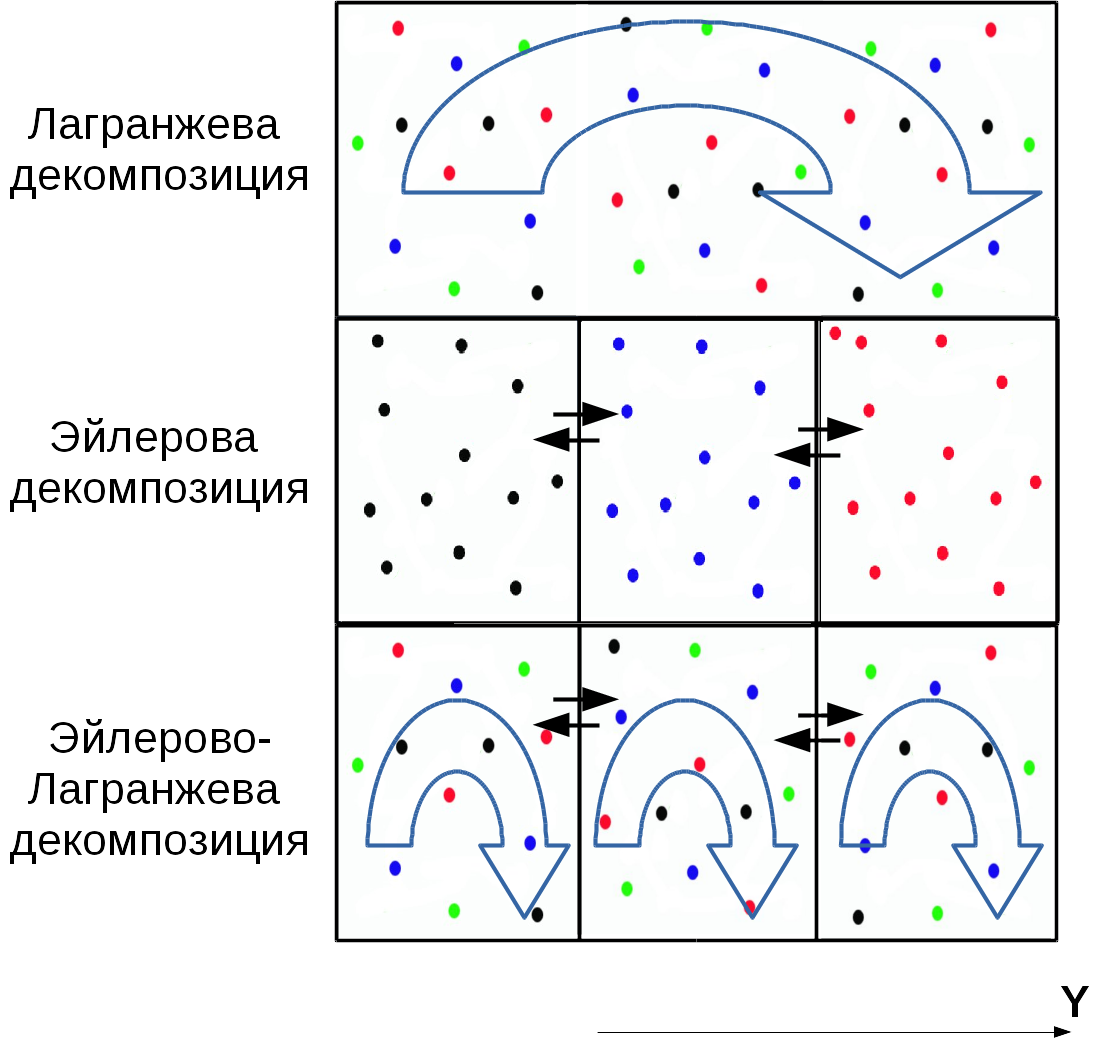
\includegraphics[height=10cm,keepaspectratio]{images/decomp_all.png}
\end{center}
\caption{Сравнение всех рассмотренных видов декомпозиции.На рисунке показано разделение расчетной области на подобласти вдоль одной из координат. Точки разных цветов показывают модельные частицы, находящиеся на разных процессорных  элементах. Маленькие черные стрелки означают обмен граничными значениями полей и токов между подобластями. Большая полая стрелка означает сборку значений тока, вычисленных каждым ПЭ по имеющимся у него частицам. Используются как  парные (MPI\_Send и MPI\_Recv), так и коллективные операции MPI (MPI\_Allreduce).}
\label{decomp_all}
\end{figure}



\clearpage

\section{Ход вычислений в программе}

Приведем \textbf{общую схему вычислений в программе}:
\begin{enumerate}
	\item Создание начального 
	распределения модельных частиц
	(выполняется независимо 
	всеми MPI-процессами) (\textbf{координаты и импульсы частиц генерируются в оперативной памяти} ). 
	\item Далее на каждом временном шаге:
	\begin{enumerate}
		\item Вычисление полей. Обмен граничными значениями полей между соседними узлами многопроцессорной ВС
		\item Вычисление сдвига модельных частиц. Вычисление токов, обмен граничными значениями токов между соседними узлами многопроцессорной ВС
		\item Выполнение диагностических процедур, вывод результатов на диск. Вывод выполняется стандартными средствами C/C++.
	\end{enumerate}	
\end{enumerate}

Приведем также
\textbf{описание выходных данных программы.}
Результатами работы являются
(опционально, каждая выдача может быть отключена):
\begin{itemize}
	\item Списки модельных частиц (координаты, импульсы)
	\item Плотности электронов, ионов и электронов пучка
	\item Электрическое и магнитное поля (все три компоненты)
	\item Ток (три компоненты)
	\item Одномерная функция распределения электронов (всех, и пучка, и плазмы) по энергии
\end{itemize}

С точки зрения тестирования ВС основное значение имеют следующие выдачи (отдельно для каждого MPI-процесса):

\begin{itemize}
	\item Средняя продолжительность операций MPI, причем по отдельности для разных объемов пересылаемых данных и разных стадий вычислительного алгоритма:
	\begin{itemize}
		\item MPI\_Send/Recv - пересылка граничных значений поля и пересылка частиц
		\item MPI\_Allreduce - сложение значений тока в подобласти при лагранжевой декомпозиции
		
	\end{itemize}	
	\item Время пересылки частиц, граничных значений поля, время сборки данных при выполнении коллективных операций   
	\item Время выполнения каждой отдельной стадии вычислительного алгоритма:
	\begin{itemize}
		\item расчет поля, 
		\item пересылка граничных значений, 
		\item расчет движения частиц, 
		\item пересылка частиц в соседние процессоры, 
		\item сборка значений тока при лагранжевой декомпозии
	\end{itemize}
	\item Время записи файлов на диск 
	\item Время копирования данных на GPU и обратно
	
\end{itemize}
Расчет производительности ВС в целом и отдельных ее элементов выполняется после выполнения программы, на основе полученных времен. 



\section{Программная реализация вычислительных методов}
   В этом разделе подробно описывается ход вычислений в программе-тесте, созданной в рамках диссертационной работы. Несмотря на то, что ни сами вычислительные методы, ни их программная реализация не являются основным содержанием диссертации, и не входят в положения, выносимые на защиту, тем не менее необходимо максимально точно описать, что входит в программу-тест, запускаемую на ВС для того, чтобы было видно, какая нагрузка создается на различные подсистемы ВС и в частности, для того, чтобы определить объем вычислений (количество операций с плавающей точкой) на каждую модельную частицу, количество данных в оперативной памяти, и объем пересылок.
   
   
\subsection{Вычисление электромагнитного поля во всей расчетной области}

На листинге \ref{list:eme} показана функция emeElement, выполняющая расчет одной из компонент электрического поля в отдельном узле сетки. Как видно на листинге, для расчета используются: соответствующая компонента тока J и две компоненты магнитного поля H1 и Н2. Вспомогательная функция getGlobalCellNumber используется для того, чтобы переходить от трехмерной нумерации узлов сетки к одномерной (все сеточные величины хранятся в виде одномерных массивов).    
\begingroup
\captiondelim{ } % разделитель идентификатора с номером от наименования
\lstinputlisting[lastline=49,language={[ISO]C++},caption={Функция, выполняющая расчет одной из компонент электрического поля в отдельном узле сетки.},label={list:eme}]{listings/emeElement.cxx}
\endgroup 
Непосредственно на листинге \ref{list:eme} можно увидеть 7 операций с плавающей точкой. Эта функция вызывается $N_X \times N_Y \times N_Z$ раз для каждой из трех компонент электрического поля, всего 
$21 N_X \times N_Y \times N_Z$ операций.

\begingroup
\captiondelim{ } % разделитель идентификатора с номером от наименования
\lstinputlisting[lastline=49,language={[ISO]C++},caption={Функция, выполняющая первый этап расчета одной из компонент магнитного поля в отдельном узле сетки.},label={list:emh1}]{listings/emhElement.cxx}
\endgroup 

 Аналогично, на листинге \ref{list:emh1} видно 7 операций с плавающей точкой. Эта функция также вызывается $N_X \times N_Y \times N_Z$ раз для каждой из трех компонент магнитного поля, всего 
 $21 N_X \times N_Y \times N_Z$ операций.

\begingroup
\captiondelim{ } % разделитель идентификатора с номером от наименования
\lstinputlisting[lastline=49,language={[ISO]C++},caption={Функция, выполняющая второй этап расчета одной из компонент магнитного поля в отдельном узле сетки.},label={list:emh2}]{listings/emh2Element.cxx}
\endgroup 
   
И листинг \ref{list:emh2} добавляет еще одну операцию. Эта функция также вызывается $N_X \times N_Y \times N_Z$ раз для каждой из трех компонент магнитного поля, всего 
$3 N_X \times N_Y \times N_Z$ операций.

В итоге вычислительная нагрузка при вычислении электромагнитного поля составляет $45 N_X \times N_Y \times N_Z$ операций.
   
  
   
\subsection{Расчет электромагнитного поля в точке нахождения модельной частицы}
На листинге \ref{list:interpolate} показана функция, интерполирующая значения электромагнитного поля из узлов ячейки в точку нахождения частицы. Как видно из листинга, поля и частицы хранятся внутри ячейки, а не в виде одного глобального массива, содержащего значения поля во всей области. Подход с хранением полей и частиц в виде глобальных массивов также был реализован, и важно отметить, что при этом возникает существенная разница по производительности. Эта разница подробно исследуется в 3-й главе (раздел \ref{procs_influence}) и обычно составляет до 200 \%. Таким образом для программы-теста можно использовать как тот, так и другой подход, внося соответствующую поправку в полученные результаты.
   
\begingroup
\captiondelim{ } % разделитель идентификатора с номером от наименования
\lstinputlisting[lastline=49,language={[ISO]C++},caption={Расчет электромагнитного поля в точке нахождения модельной частицы},label={list:interpolate}]{listings/interpolate.cxx}
\endgroup 
Интерполяционные коэффициенты, задаваемые в качестве параметров функции Interpolate, вычисляются в функции InverseKernel, реализующей операцию, обратную по отношению к ядру модельной частицы (листинг \ref{list:inverse}):

\begingroup
\captiondelim{ } % разделитель идентификатора с номером от наименования
\lstinputlisting[lastline=32,language={[ISO]C++},caption={Вычисление интерполяционных коэффициентов},label={list:inverse}]{listings/inverse.cxx}
\endgroup    

\subsection{Расчет движения модельной частицы}
В этом разделе на листинге \ref{list:push} показана функция, рассчитывающая движение модельной частицы, то что в зарубежной литературе именуется particle pusher. Следует отметить, что это наиболее важная с точки зрения производительности и наиболее вычислительно нагруженная часть программы.

\begingroup
\captiondelim{ } % разделитель идентификатора с номером от наименования
\lstinputlisting[lastline=79,language={[ISO]C++},caption={Интегрирование уравнений движения модельной частицы},label={list:push}]{listings/push.cxx}
\endgroup   
 
Цель демонстрации всех перечисленных фрагментов программного кода, заключается в том, чтобы можно было подтвердить оценку количества операций с плавающей точкой, затрачиваемых на одну модельную частицу в течение одного временного шага: 500 операций. Это число будет в дальнейшем использоваться для определения производительности вычислительных систем и в частности, их процессорных ядер во флопсах (FLOPS).  


\section{Список входных и выходных данных программы}	

Входные данные:
\begin{itemize}
\item Размер сетки
\item Количество процессоров
\item Количество частиц в ячейке
\item Размер области
\item Размер части области, занятой пучком и плазмой
\item Внешнее магнитное поле
\item Энергия частиц пучка
\item Поперечная температура частиц пучка
\item Температура плазмы (X,Y,Z)
\end{itemize}

Выходные данные (опционально, каждая выдача может быть отключена):
\begin{itemize}
\item Списки модельных частиц (координаты, импульсы)
\item Плотности электронов, ионов и электронов пучка
\item Электрическое и магнитное поля (все три компоненты)
\item Ток (три компоненты)
\item Одномерная функция распределения электронов (всех, и пучка, и плазмы) по энергии
\end{itemize}

С точки зрения тестирования ВС основное значение имеют следующие выдачи (отдельно для каждого MPI-процесса):

\begin{enumerate}
	\item Средняя продолжительность операций MPI, причем по отдельности для разных объемов пересылаемых данных и разных стадий вычислительного алгоритма:
	\begin{itemize}
		\item MPI\_Send/Recv - пересылка граничных значений поля и пересылка частиц
		\item MPI\_Allreduce - сложение значений тока в подобласти при лагранжевой декомпозиции
		
	\end{itemize}	
	\item Время пересылки частиц, граничных значений поля, время сборки данных при выполнении коллективных операций   
	\item Время выполнения каждой отдельной стадии вычислительного алгоритма:
	\begin{itemize}
		\item расчет поля, 
		\item пересылка граничных значений, 
		\item расчет движения частиц, 
		\item пересылка частиц в соседние процессоры, 
		\item сборка значений тока при лагранжевой декомпозиции
	\end{itemize}
	\item Время записи файлов на диск 
	\item Время копирования данных на GPU и обратно
	
\end{enumerate}



